% Four exact intersections for a=4, A=1, c=2: (+/-2,+/-3)
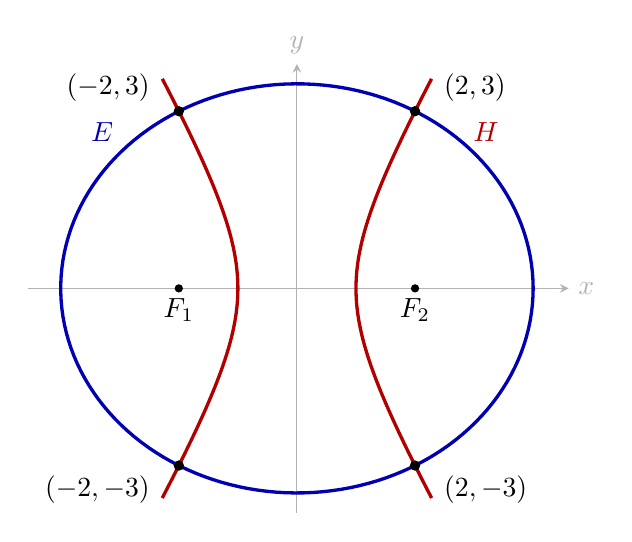
\begin{tikzpicture}[scale=0.75,>=stealth]
 \draw[->,gray!60] (-4.55,0)--(4.6,0) node[right]{$x$};
 \draw[->,gray!60] (0,-3.8)--(0,3.8) node[above]{$y$};
 \draw[blue!70!black,very thick,samples=160,domain=0:360,variable=\t]
  plot ({4*cos(\t)},{sqrt(12)*sin(\t)});
 \draw[red!70!black,very thick,samples=110,domain=-3.55:3.55,variable=\t]
  plot ({sqrt(1+\t*\t/3)},{\t});
 \draw[red!70!black,very thick,samples=110,domain=-3.55:3.55,variable=\t]
  plot ({-sqrt(1+\t*\t/3)},{\t});
 \foreach \x/\y in {2/3,2/-3,-2/3,-2/-3}{\fill[black] (\x,\y) circle (2.5pt);}
 \node[above right,xshift=7pt] at (2,3) {$(2,3)$};
 \node[below right,xshift=7pt] at (2,-3) {$(2,-3)$};
 \node[above left,xshift=-7pt] at (-2,3) {$(-2,3)$};
 \node[below left,xshift=-7pt] at (-2,-3) {$(-2,-3)$};
 \fill (-2,0) circle (2pt) node[below]{$F_1$};
 \fill (2,0) circle (2pt) node[below]{$F_2$};
 \node[blue!70!black] at (-3.3,2.65) {$E$};
 \node[red!70!black] at (3.2,2.65) {$H$};
\end{tikzpicture}
